\documentclass[11pt]{article}
\usepackage{eadca-template}
\usepackage[plain]{algorithm}

\usepackage[brazil,english]{babel}
\usepackage[utf8]{inputenc}
\usepackage[T1]{fontenc}

\usepackage{graphicx,url}
\usepackage[hang]{subfigure}
\usepackage{psfrag}

\sloppy


\title{Instruções para Autores}

\author{Autores \and Nome\_Orientador}
\address{\email{\{autores,Nome\_Orientador@dca.fee.unicamp.br\}}}

\begin{document}

\hyphenation{}
\pagestyle{fancy}

%%%%%%%%%%%%%%%%%%%%%%%%%%%%%%%%%%%%%%%%%%%%%%%%%%%%%%%%%%%%%%%%%%%%%%%%%%%%%
\twocolumn[
\maketitle
\thispagestyle{fancy}
\selectlanguage{english}

   \begin{abstract}
			This article gives some guidelines for preparing a two-column paper.  \textbf{Its abstract must be written in English or Portuguese} and is limited to 150 words. It should be a fully self-contained description of your work, conveying motivation, problem statement, the way that you plan to solve/have solved your problem, expected/achieved/on-the-road results, and the implications of your results. It is a way to convince people that it is worth taking their time to acquire and read the rest of the paper. We exceptionally cite~\cite{Koop97} in this abstract for further reading.
   \end{abstract}

  \keywords{They must be in English or Portuguese. Put here keywords that people looking for your paper might use or that may help the review committees or editors assign it to appropriate reviewers.}

]
%%%%%%%%%%%%%%%%%%%%%%%%%%%%%%%%%%%%%%%%%%%%%%%%%%%%%%%%%%%%%%%%%%%%%%%%%%%%%
\selectlanguage{brazil}

  \section{Introdu\c{c}\~{a}o}
  \label{sec:introducao}

   Os trabalhos, que podem ser escritos tanto em portugu\^{e}s quanto em
   ingl\^{e}s, devem conter uma introdu\c{c}\~{a}o, a sua proposta de
   pesquisa, os resultados esperados e/ou j\'{a} obtidos, conclus\~{o}es e uma
   lista de refer\^{e}ncias bibliogr\'{a}ficas. Cada trabalho deve ter, no
   m\'{a}ximo, \textbf{duas p\'{a}ginas}, caso seja um \textbf{resumo expandido}, ou \textbf{quatro p\'{a}ginas}, caso seja um \textbf{trabalho completo}, incluindo figuras, tabelas e demais itens
   complementares. Os tipos e tamanhos das fontes, assim como as
   margens e os diversos estilos necess\'{a}rios, devem corresponder aos
   apresentados neste documento.

   Na introdu\c{c}\~{a}o, voc\^{e} deve expor com clareza as motiva\c{c}\~{o}es
   subjacentes ao problema tratado em seu artigo, mostrando aos seus
   leitores a import\^{a}ncia do tema. Se o seu trabalho se insere em um
   assunto mais amplo, pode ser interessante que voc\^{e} sintetize este
   assunto antes de especificar o seu problema. Um pequeno resumo
   sobre como o seu problema tem sido estudado pelos outros
   pesquisadores tamb\'{e}m pode contribuir para situar o seu
   trabalho~\cite{Blinn87}. Em alguns casos, \'{e} v\'{a}lido incluir na
   introdu\c{c}\~{a}o as conjecturas ou hip\'{o}teses que ajudar\~{a}o a guiar as
   suas investiga\c{c}\~{o}es.

  %%%%%%%%%%%%%%%%%%%%%%%%%%%%%%%%%%%%%%%%%%%%%%%%%%%%%%%%%%%%%%%%%%%%%%%%%%%%%
  \section{Proposta}
  \label{sec:detalhes}

  A proposta deve ser objetiva, ou seja, nela devem ser destacadas as
  id\'{e}ias-chave.  Recursos complementares, como diagramas e figuras,
  podem ajudar na explana\c{c}\~{a}o das suas id\'{e}ias.  Fluxogramas s\~{a}o boas
  alternativas para apresentar um procedimento, grafos ajudam a
  visualizar as rela\c{c}\~{o}es entre os objetos de interesse e imagens
  bonitas sempre chamam aten\c{c}\~{a}o.

   Ao escrever a sua proposta, procure utilizar uma linguagem clara e
   objetiva. Frases curtas e em ordem direta s\~{a}o mais recomendadas
   para textos cient\'{\i}ficos. Repeti\c{c}\~{o}es de palavras ou de id\'{e}ias devem
   ser evitadas. Vale lembrar que, hoje em dia, a maioria dos
   processadores de texto cont\'{e}m corretores ortogr\'{a}ficos. Portanto,
   erros de grafia e digita\c{c}\~{a}o podem ser facilmente
   eliminados. Recomendamos a leitura do artigo do Prof. Rog\'{e}rio
   Lacaz-Ruiz~\cite{LR}, que d\'{a} algumas no\c{c}\~{o}es a cerca reda\c{c}\~{a}o de um texto
   cient\'{\i}fico.

  Nesta se\c{c}\~{a}o, apresentamos detalhes da formata\c{c}\~{a}o dos artigos do
  Encontro de Alunos e Docentes do DCA (EADCA).


\subsection{P\'{a}ginas}
\label{sec:paginas}

As p\'{a}ginas {\bf n\~{a}o devem ser numeradas}. As medidas de formata\c{c}\~{a}o
s\~{a}o: folha A4; margem superior: 2,3 cm; margem inferior: 2 cm;
margem esquerda: 1,5 cm; margem direita: 1,5 cm. O texto deve ser em
duas colunas, separadas por um espa\c{c}o de 0,6 cm. A fonte \'{e} {\it Time
News Roman\/} 11pt.

A primeira p\'{a}gina deve conter o t\'{\i}tulo do trabalho, nomes dos autores, um resumo ({\it abstract}) e um conjunto de
palavras-chave ({\it keywords}) \textbf{no idioma escolhido para o trabalho}. O t\'{\i}tulo de cada se\c{c}\~{a}o ou subse\c{c}\~{a}o deve
estar em negrito. Procure evitar se\c{c}\~{o}es com uma \'{u}nica
subse\c{c}\~{a}o: usualmente, ela pode ser substitu\'{\i}da por par\'{a}grafos sem comprometer a qualidade do texto.


\subsection{Figuras e Legendas}
\label{sec:figuras}

As figuras s\~{a}o, de certa forma, complementares a seu texto.  Portanto,
elas devem ser citadas, e o texto contido nelas deve ser na mesma
l\'{\i}ngua. Elas poder\~{a}o ocupar uma ou duas colunas.  Abaixo de cada
figura devem ser colocados o seu n\'{u}mero e uma legenda.  Adote uma
numera\c{c}\~{a}o \'{u}nica para o documento todo e centralize as legendas, em
conson\^{a}ncia com o modelo da Figura~\ref{fig:forma_de_onda}, que traz o
gr\'{a}fico de uma fun\c{c}\~{a}o senoidal.

  \begin{figure}[H]
        {\centering
        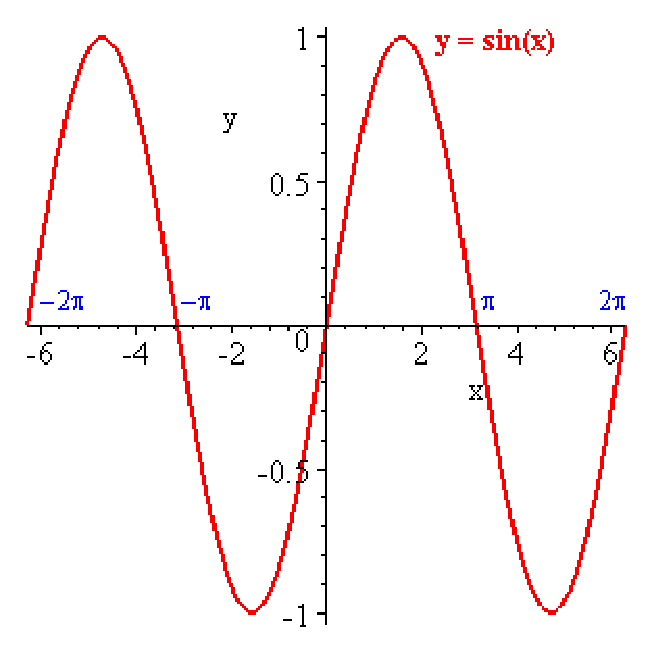
\includegraphics[height=35mm]{sin.ps}
        \caption{Forma de onda senoidal.}
        \label{fig:forma_de_onda}\par}
  \end{figure}

\subsection{Tabelas}
\label{ssec:tabelas}

A formata\c{c}\~{a}o das tabelas segue a mesma recomenda\c{c}\~{a}o das figuras.
A Tabela~\ref{tab:ex} ilustra o uso de uma tabela. Esta tabela sintetiza
o tempo, em meses, que cada grupo $G_i$ necessitou para realizar a
tarefa $T_j$.

\begin{table}[H]
  {\centering
  \begin{tabular}{|c|c|c|c|c|}
  \hline
   & $G_1$ & $G_2$ & $G_2$ & $G_3$ \\
  \hline
  $T_1$ & 2 & 4 & 6 & 8 \\
  \hline
  $T_2$ & 3 & 6 & 9 & 12 \\
  \hline
  \end{tabular}
\caption{Exemplo de uma tabela.}
\label{tab:ex}
\par}
\end{table}

\subsection{Equa\c{c}\~{o}es}
\label{ssec:equacoes}

Na maioria dos textos t\'{e}cnicos, equa\c{c}\~{o}es s\~{a}o fundamentais. Elas podem ser \'{u}teis para expressar de forma
concisa o modelo de um problema. Lembre-se, no entanto, de que elas s\'{o} podem ser devidamente compreendidas
pelos seus leitores se voc\^{e} explicar o significado de cada letra que aparece nelas. Procure ainda uniformizar
as nota\c{c}\~{o}es para reduzir o esfor\c{c}o mental requerido para guardar o significado de todas as letras que
aparecem ao longo do seu artigo. Algumas dicas do emprego de equa\c{c}\~{o}es e nota\c{c}\~{o}es matem\'{a}ticas num texto
t\'{e}cnico s\~{a}o dadas em~\cite{K99}.

Como as figuras, as equa\c{c}\~{o}es devem ser complementares a seu texto, ou
seja, elas devem ser citadas, centradas e numeradas com uma numera\c{c}\~{a}o
\'{u}nica. Para exemplificar, mostramos na Eq.~\ref{eq:lagrange} uma
express\~{a}o que descreve a din\^{a}mica de um ponto no espa\c{c}o.
  \begin{equation}
  \label{eq:lagrange}
  f(x,t) = m \frac{d^2x}{dt^2},
  \end{equation}
onde $f(x,t)$ \'{e} a for\c{c}a aplicada no ponto $x$ no instante $t$ e $m$
corresponde \`{a} massa concentrada em $x$.

\subsection{Cita\c{c}\~{o}es e Refer\^{e}ncias Bibliogr\'{a}ficas}

As cita\c{c}\~{o}es devem ser por refer\^{e}ncia num\'{e}rica e as refer\^{e}ncias devem
ser completas e uniformes, organizadas pela ordem alfab\'{e}tica do
sobrenome.

\section{Resultados}

Deve-se evitar afirma\c{c}\~{o}es vagas, como ``\'{e} melhor'', ``\'{e} mais r\'{a}pido''
ou ``\'{e} mais eficiente''. Os leitores podem, por si mesmos, concluir isso,
se voc\^{e} apresentar tabelas ou gr\'{a}ficos sintetizando os seus resultados
quantitativos e os de outras propostas com objetivos similares aos
seus.

Quando n\~{a}o for poss\'{\i}vel apresentar os resultados de forma
quantitativa, utilize imagens de boa qualidade para facilitar an\'{a}lises
qualitativas.

\section{Conclus\~{o}es}

Nas conclus\~{o}es, \'{e} importante retomar o problema mencionado na
se\c{c}\~{a}o~\ref{sec:introducao} e sintetizar contribui\c{c}\~{o}es e perspectivas.
Uma boa conclus\~{a}o pode, eventualmente, inspirar outros pesquisadores a
se dedicarem a linhas relacionadas \`{a}s de seu trabalho.

Neste artigo apresentamos algumas recomenda\c{c}\~{o}es com a finalidade de
ajudar os potenciais escritores a preparar os seus manuscritos para o
EADCA. Esperamos receber uma grande quantidade de submiss\~{o}es com
qualidade.

%%%%%%%%%%%%%%%%%%%%%%%%%%%%%%%%%%%%%%%%%%%%%%%%%%%%%%%%%%%%%%%%%%%%%%%%%%%%%
  \bibliographystyle{plain}

   \bibliography{bib-template}

\end{document}
